%% -*- coding:utf-8 -*-

\chapter{树邻接语法}
\label{Kapitel-TAG}

\newcommand{\dotted}[0]{\makedash{2pt}}
\newcommand{\g}[1]{{\footnotesize $#1$}}

树邻接语法(TAG)
\isc{树邻接语法(TAG)|(}\is{Tree Adjoining Grammar (TAG)|(}
是美国宾夕法尼亚大学的Aravind Joshi提出来的一套语法理论\citep*{JLT75a-u}。
在宾夕法尼亚大学,Aravind Joshi和Anthony Kroch指导了几篇优秀的博士论文(如\citealp{Rambow94a})。
其他的重要的开展TAG研究的科研院所包括:巴黎第七大学(Anne Abeill\'{e})、美国的哥伦比亚大学(Owen Rambow)和德国杜塞尔多夫大学(Laura Kallmeyer)。
\citew{Rambow94a}和\citew{Gerdes2002b-u}针对德语展开的研究\footnote{%
  因为我对法语了解有限,所以此处我仅仅援引一些法语文献而不对其内容进行讨论。
}。
%Viola: \todostefan{leaves a little oder much - something wie als nettes Understatement im Deutschen passt hier leider nicht :-)}

从表示能力的角度来看,TAG和它的一些扩展性变体相对精确地展现了人类在理解和处理语言的时候做了什么,这也是这种语法理论能够吸引大量研究人员注意的主要原因。为了便于和上下文无关文法
\isc{上下文无关文法}\is{context"=free grammar}(Type-2 languages)形成对应,广义短语结构语法\indexgpsgc 在设计之初就对表示能力施加了很多限制,即便如此,事实上,GPSG在这方面仍然问题多多\citep{Shieber85a,Culy85a}\footnote{%
  参阅\citet{Pullum86a}以了解关于复杂性的讨论,参阅G.\ \citew{GMueller2011a}以了解针对德语的非上下文无关性的讨论,
  这种分析和Culy分析N-P-N构式的工作具有一定的相似性。(参阅\ref{Abschnitt-NPN-Konstruktion})%
   }。像HPSG\indexhpsgc 和CxG\indexcxgc 这样的语法理论可以产生/描写所谓的0-型语言,相较于目前我们所假设的自然语言的复杂度,其描写能力过强。
目前通行的假设认为自然语言的复杂度位于上下文无关
\isc{复杂类型}\is{complexity class}
\isc{上下文无关文法}\is{context"=free grammar}和上下文相关
\isc{上下文相关文法}\is{context"=sensitive grammar} (1-型) 语言之间。这个类被称为“弱上下文相关”(mildly context sensitive)。\isc{弱上下文相关}\is{mildly context"=sensitive grammar}一些TAG变体处于这个语言类中,一种假设认为他们恰好产生出自然语言中的结构,不多也不少。
欲了解更多的关于复杂度的讨论,可以参见\ref{Abschnitt-Kompetenz-Performanz-TAG}和\ref{sec-generative-capacity}。

有各种各样的系统可以处理TAG语法\citep*{DHSSX2000a-u,PKMLD2008a-u,KLMPDE2008a-u,Koller2017a-u}。
针对下列语言也开发了或大或小的TAG语法片段:
\begin{itemize}
\item 阿拉伯语\il{Arabic} \citep*{ArabTAG2008a},
\item 德语\citep{Rambow94a,Gerdes2002a,KY2004b,Lichte2007a},
\item 英语\il{English} \citep{XTAG2001a,Frank2002a-u,KrochJoshi87a-u},
\item 法语\il{French} \citep{Abeille88a,Candito96a,Candito98a,Candito99a-u,Crabbe2005a-u},
\item 意大利语\il{Italian} \citep{Candito98a,Candito99a-u},%,Kinyon2003a}
\item 韩语\il{Korean} \citep*{HYKP2000a-u,KY2004b},
\item 越南语\il{Vietnamese} \citep*{VietnameseTAG2008a}
%\item Tagalog\il{Tagalog} \citep{MR2003a}
\end{itemize}
\citet{Candito96a}开发了一个可以表示元语法(meta grammar)的系统,针对跨语言描写,它允许使用一个统一的规范。上述针对特定语言的语法,有一些是基于这个系统开发的。如\citet*{KSYJ2006a}基于一个公共元语法得到了针对动词位于第二位语言(verb second languages)的语法。这其中就包括了第一个依地语(Yiddish\il{Yiddish})的TAG语法。

\citet{Resnik92a}研究了如何将TAG和一个统计
\isc{统计学}\is{statistics}模块耦合在一起。

\section{关于表示形式的一般说明}
\label{sec-tag-allgemein}

\subsection{配价信息的表示}

图\vref{abb-elementare-Baeume}
\isc{价|(}\is{valence|(}展示了被称之为基本树(elementary trees)
\isc{基本树}\is{elementary tree}的结构。
基本树出现在词典中,可以通过组合构建更大的树。
\begin{figure}
\hfill
\begin{forest}
tag
[NP
	[John;John]]
\end{forest}
\hfill
\begin{forest}
tag
[S
	[NP$\downarrow$]
	[VP
		[V
			[laughs;笑]]]]
\end{forest}
\hfill
\begin{forest}
tag
[VP
	[ADV
		[always;总是]]
	[VP*]]
\end{forest}
\hfill\mbox{}
\caption{\label{abb-elementare-Baeume}基本树}
\end{figure}%
%
待插入论元的结点用特殊标记进行标识(laugh树中的NP$\downarrow$
\isc{$\downarrow$}\is{$\downarrow$})。
作为附接语插入的结点也用特殊标记进行标识(always树中的VP$^*$
\isc{*}\is{*})。
如果语法中的每一个基本树都至少含有一个词的话,则称之为词汇化树邻接语法({Lexicalized Tree Adjoining Grammar},简称LTAG)。
\isc{价|)}\is{valence|)} 

\subsection{替换}

图\vref{abb-Substitution}
\isc{替换|(}\is{substitution|(}展示了如何进行结点的替换。
\begin{figure}
\centerline{%
\begin{forest}
tag
[S
	[NP$\downarrow$,
          [NP, substitution
            [John;John]]]
	[VP
		[V
			[laughs;笑]]]]
\end{forest}
\hspace{1em}
$\leadsto$
\hspace{1em}
\begin{forest}
tag
[S
	[NP
		[John;John]]
	[VP
		[V
			[laughs;笑]]]]
\end{forest}
}
\caption{\label{abb-Substitution}替换}
\end{figure}%
其它的子树必须插入待替换结点,如laughs子树中的NP结点。
在这个例子中,John的子树就插入到了相应的位置。
\isc{替换|)}\is{substitution|)}

\subsection{附接语}

图\vref{abb-Adjunktion}
\isc{附接|(}\is{adjunction|(}
\isc{附接语|(}\is{adjunct|(}展示了always的附接树(adjunction tree)是如何被使用的。

%
\begin{figure}
\centerline{%
\begin{forest}
tag
[S
	[NP
		[John;John]]
	[VP
		[V
			[laughs;笑]]]]
\end{forest}
\hspace{0.5cm}
\begin{forest}
tag
[VP
	[ADV
		[always;总是]]
	[VP*]]
\end{forest}
\hspace{1em}
$\leadsto$
\hspace{1em}
\begin{forest}
tag
[S
	[NP
		[John;John]]
	[VP
		[ADV
			[always;总是]]
		[VP
			[V
				[laughs;笑]]]]]
\end{forest}
}
\caption{\label{abb-Adjunktion}附接}
\end{figure}%
附接树可以插入其它的树中。在插入时,目标结点(和标有`*'的结点一样的范畴)被附接树替换。
\isc{附接语|)}\is{adjunction|)}
\isc{附接|)}\is{adjunct|)}

TAG和我们之前在第\ref{Kapitel-PSG}章遇到的简单短语结构语法有一个显著不同,即树的范围扩大了:例如,laugh树中有一个不是动词兄弟结点的NP结点。在短语结构语法(当然包括了GB\indexgbc 和GPSG\indexgpsgc,因为这两个理论或多或少都依赖于短语结构语法)中,我们只能描写深度为一的子树。对于laughs的子树而言,相应的规则如(\mex{1})所示:
\ea
\begin{tabular}[t]{@{}l@{ }l}
S  & $\to$ NP VP\\
VP & $\to$ V\\
V  & $\to$ laughs\\
\end{tabular}
\z
在讨论TAG时,一个常常提及的概念是局部域({locality domains})
\isc{定域}\is{locality}。
扩展的局部域在分析习语时有着重要作用(参见\ref{Abschnitt-Diskussion-Lokalitaet})。

TAG和其它的语法理论不同的地方在于它允许结构被再次打散。
基于这种方式,我们可以使用附接操作向一个给定的树中不断添加新成分,其结果是原本邻接于一处的组成成分在最终所构造出来的树中相隔可以任意远。
我们将在\ref{TAG-Fernabh}中看到,这个性质对于脱离移位去分析长距离依存非常重要。

\subsection{语义}

基于TAG,处理句法语义接口有不同的方法。
如为树中的每一个结点都分配一个语义表征,也可以选择给每一棵基本树分配一个语义表征。
语义的构建过程利用的不是句法结构本身的信息而是关于句法结构是如何构造出来的信息。
这种方法首先由\citet{CK98a}提出,而后\citet{KJ2003a}继续研究了这种思路。
我们接下来介绍一下基本的处理机制。

%\begin{sloppypar}
讨论TAG的文献经常区分两种树——导出树与推导树
\isc{推导树}\is{derivation tree}。
导出树对应于组成成分结构(也就是图\ref{abb-Substitution}和\ref{abb-Adjunktion}中的“John laughs”以及“John always laughs”所对应的树)。
而推导树则包含了推导的历史,也就是如何将基本树组合在一起的信息。
推导树中的元素表示了谓词论元依存关系(predicate"=argument dependency),这也是为什么可以通过推导树进行语义推导的原因。
基于(\mex{1})我们来介绍这样的分析过程。
%\end{sloppypar}

\ea
\gll Max likes Anouk.\\
Max 喜欢 Anouk\\
\glt `Max喜欢Anouk。'
\z
(\mex{0})的基本树和导出树如图\vref{Abbildung-Max-likes-Anouk}所示。
\begin{figure}
\centering
\begin{forest}
tag
[S
	[NP$\downarrow$
          [NP,substitution [Max;Max]]]
	[VP
		[V
			[likes;喜欢]]
		[NP$\downarrow$
                  [NP,substitution [Anouk;Anouk] ]]]]
\end{forest}
\hspace{1em}
$\leadsto$
\hspace{1em}
\begin{forest}
tag
[S
	[NP
		[Max;Max]]
	[VP
		[V
			[likes;喜欢]]
		[NP
			[Anouk;Anouk]]]]
\end{forest}
\caption{\label{Abbildung-Max-likes-Anouk}“Max likes Anouk.”中的基本树与导出树}
\end{figure}%
树中的结点按照从上到下、从左到右的顺序进行编号。likes树中的结点按照这种方式编号后的结果如图\vref{Abbildung-Knotenpositionen}所示。
树中最高的结点为S,其位置编号为0。在S之下有一个NP和一个VP结点。这些结点同样从0开始计数。\todostefan{Timm: Noch üblicher ist es vielleicht, mit 1 anzufangen. D.h. nur der Wurzelknoten hat die Adresse 0.}NP为位置0,而VP为1。VP结点同样有两个子结点:V和宾语NP。V编号0,而宾语NP为1。将这些编号组合起来,我们就可以无歧义地指称树中的任意独立元素。主语位置的NP为00,因为它是S的一个子结点且出现在第一的位置上。宾语位置的NP为011,因为它在S(0)之下的VP(S的第二个子结点,为1)中,且出现在第二的位置上(VP的第二个子结点,为1)。

\begin{figure}
\centerline{%
\begin{forest}
tag
[S {(0)}
	[NP$\downarrow$ {(1)}]
	[VP {(2)}
		[V {(2.1)}
			[likes;喜欢]]
		[NP$\downarrow$ {(2.2)}]]]
\end{forest}
}
  \caption{\label{Abbildung-Knotenpositionen}likes树中结点的位置}
\end{figure}%

有了这些位置,(\mex{0})的导出树就可以用图\vref{Abbildung-Ableitungsbaum}进行表示。
\begin{figure}
\centerline{%
\begin{forest}
[likes, l sep+=1em
	[Max,edge label={node[midway,left]{1~~}}]
	[Anouk,edge label={node[midway,right]{~2.2}}]]
\end{forest}
}
\caption{\label{Abbildung-Ableitungsbaum}“Max likes Anouk.”的推导树}
\end{figure}%
推导树表示了这样的事实:likes的基本树可以和两个论元相结合,这两个论元分别在位置00和011处做替换。
究竟是什么样的东西放置到了这两个结点上?推导树也包含了上述信息。

\citet{KJ2003a}使用了一种最小递归语义\citep*{CFPS2005a}\indexmrsc 的变体作为他们的语义表征范式。
和对HPSG中的语义进行阐释时(\ref{Abschnitt-HPSG-Semantik})一样,我在这里将采用明确简化的表示方式。
对我们假定Max、likes和Anouk的基本树的语义表征为(\mex{1})。 
\ea
基本树的语义表征:\\*
\begin{tabular}[t]{|l|}\hline
max(x)\\\hline
arg: $-$\\\hline
\end{tabular}
\hfill
\begin{tabular}[t]{|l|}\hline
like(x$_1$, x$_2$)\\\hline
arg: \sliste{ x$_1$, 1 }, \sliste{ x$_2$, 2.2 }\\\hline
\end{tabular}
\hfill
\begin{tabular}[t]{|l|}\hline
anouk(y)\\\hline
arg: $-$\\\hline
\end{tabular}
\hfill\mbox{}
\z
在一个替换操作中,一个变量会被赋予一个值。例如,如果将Max的基本树插入到likes子树的主语位置,那么x$_1$就等于x。
同样道理,如果Anouk的树被插入到宾语位置,x$_2$等于y。
这些组合的结果如(\mex{1})所示:
\eas
基本树的语义的组合:\\
\begin{tabular}[t]{|l|}\hline
like(x, y)\\
max(x)\\
anouk(y)\\\hline
arg: $-$\\\hline
\end{tabular}
\zs

\noindent
多元成分LTAG(Multi-Component LTAG)
\isc{多成分树邻接语法}\is{Multi-Component TAG}是TAG的一个扩展,\citet{KJ2003a}展示了如何基于它
处理量词作用域
\isc{辖域}\is{s\textsc{cop}e}的问题,他们也讨论了嵌入动词的复杂情况。感兴趣的读者可以阅读他们的原始论文。

\section{局部语序重列}
\label{Abschnitt-MC-TAG}\label{sec-ld-lp-tag}

\isc{成分序列|(}\is{constituent order|(}TAG中,每一个词都对应一族树。为了解释不同的语序,我们可以利用不同的树来对应不同的语序,如假定双宾及物动词对应于六棵子树,每棵子树都对应于一种不同的论元位置安排。我们可以通过词汇规则
\isc{词汇规则}\is{lexical rule}来建立树之间的关联。这种基于词汇规则的分析类似\citet{Uszkoreit86b}基于范畴语法的分析。

另外一种方法是参照我们在GPSG一章讨论过的ID/LF形式
\isc{ID/LP语法}\is{ID/LP grammar}假设,为TAG设立类似的形式。\citet{Joshi87b}把支配结构和序列线性化限制捆绑在一起,定义为一个基础结构。不同于GPSG,序列线性化规则仅仅对一部分支配结构起作用,并非对所有的支配规则都成立。这也类似我们在\ref{sec-ECG}里看到的体验构式语法分析。图\vref{Abbildung-TAG-S}是一个带有结点序的支配树。
\begin{figure}
\centerline{%
$\alpha$ = \begin{forest}
baseline, tag
[S$_0$
	[NP$_1$]
	[VP$_2$
		[V$_{2.1}$]
		[NP$_{2.2}$]]]
\end{forest}
}
\caption{\label{Abbildung-TAG-S}带有结点序的支配关系}
\end{figure}%
如果我们把支配关系和(\mex{1})中的线性化规则进行结合,我们可以得到和我们在一般的短语结构规则里一样的语序,即NP$_1$ V NP$_2$。
\ea
LP$^\alpha_1$ = \{ 1 $<$ 2, 2.1 $<$ 2.2 \}
\z
如果我们按照(\mex{1})来约束序列线性化,(\mex{2})中所有的语序都是被允准的,因为空集意味着我们没有施加任何限制。
\ea
LP$^\alpha_2$ = \{ \}
\z
\eal
\ex NP$_1$ V NP$_2$
\ex NP$_2$ V NP$_1$
\ex NP$_1$ NP$_2$ V 
\ex NP$_2$ NP$_1$ V
\ex V NP$_1$ NP$_2$
\ex V NP$_2$ NP$_1$ 
\zl
不考虑结构成分的层次性,即树中含有NP与VP一层,GPSG\indexgpsgc 定义的扁平句子规则所定义的全部语序都可以由上述TAG方法复现。
因为支配关系包括了更大的局部域,这样的语法也称为LD/LP语法(local dominance/linear precedence),而非ID/LP语法(immediate dominance/linear precedence)\citep*{JSW90a-u}。

\S \ref{sec-tag-allgemein}所介绍的简单的TAG变体并不能处理不同动词的论元被杂列时的语序问题,如(\mex{1})。
\ea
\label{ex-weil-ihm-das-Buch-jemand-zu-lesen-versprochen-hat-drei}
\gll weil    ihm das Buch jemand   zu lesen versprochen hat\footnotemark\\
%     because him.\dat{} the.\acc{} book somebody.\nom{} to read promised has\\
     因为 他.\dat{} \textsc{det}.\acc{} 书 有些人.\nom{} \textsc{inf} 读 保证 \textsc{aux} \\
\footnotetext{%
\citew{Bech55a}介绍了更多的关于这种语言现象的例子。
}
%\glt `because somebody promised him to read the book'
\glt `因为有人向他保证读这本书'
\z
在(\mex{0})中, das Buch(这本书)是zu lesen(读)的宾语,ihm(他)和jemand(有个人)分别是versprochen(保证)和hat(\textsc{aux})的依赖词。这些例子可以用\citet{Joshi87b}提出来的LD/LP"=TAG进行分析,也可以用自由序TAG(Free Order TAG,简称FO"=TAG
\isc{TAG!自由语序树邻接语法(FO-TAG)}\is{TAG!Free Order (FO"=TAG)})\citep*[\page 21]{BJR91a}进行分析,二者都允许表示依存关系的边交叉。
\isc{投射性}\is{projectivity}

因为某些限制在FO"=TAG中不能很好地表示\citep[\page 48--50]{Rambow94a},研究者又提出了多元成分TAG(Multi"=Component TAG)。
\isc{多成分树邻接语法}\is{Multi-Component TAG}
\isc{树邻接语法(TAG)!多成分树邻接语法(MC-TAG)|(}\is{Tree Adjoining Grammar (TAG)!Multi"=Component (MC-TAG)|(} 
\citet*{JBR2000a}用(\mex{1})中的例子阐释了简单的LTAG语法在处理(\mex{0})这样的句子时所存在的问题\footnote{%
  作者们采用了versprochen hat而不是versprach,这听起来好一些但却并没有对应到他们所使用的树上。
}:
\eal
\ex 
\gll \ldots{} daß  der        Detektiv  dem        Klienten [den Verdächtigen des Verbrechens zu überführen] versprach\\
%         {}   that the.\nom{} detective the.\dat{} client   \spacebr{}the.\acc{} suspect the.\gen{} crime to indict promised\\
{}  \textsc{comp}  \textsc{det}.\nom{} 探员 \textsc{det}.\dat{} 委托人   \spacebr{}\textsc{det}.\acc{} 嫌疑人 \textsc{det}.\gen{} 犯罪 \textsc{inf} 起诉 保证\\
%  \glt `that the detective promised the client to indict the suspect of the crime'
  \glt `探员向客户保证会起诉犯罪活动的嫌疑人'
\ex\label{Beispiel-Joshi-NP4} 
\gll \ldots{} daß  des        Verbrechens$_k$ der        Detektiv  den Verdächtigen$_j$~~~ dem         Klienten [\_$_j$ \_$_k$ zu überführen] versprach\\
{}     \textsc{comp}  \textsc{det}.\gen{} 犯罪           \textsc{det}.\nom{} 探员 \textsc{det}.\acc{} 嫌疑人   \textsc{det}.\dat{}  委托人   {}      {}     \textsc{inf} 起诉  保证\\
\zl
相关动词的LTAG基本树参见图\vref{Abbildung-Kontrollverben-TAG}。
\begin{figure}
\oneline{%
\begin{forest}
tag, baseline
[S
	[NP$_2^2\downarrow$]
	[S
		[NP$_2^1\downarrow$]
		[S
			[NP
				[PRO]]
			[VP
				[NP$_2^1$
					[e]]
				[NP$_2^2$
					[e]]
				[V$_2$
					[zu überführen;\textsc{inf} 起诉]]]]]]
%					[zu überführen;\textsc{inf} 起诉to indict]]]]]]
\end{forest}
\begin{forest}
tag, baseline
[S
	[NP$_1^1\downarrow$]
	[VP
		[NP$_1^2\downarrow$]
		[S*]
		[V$_1$
		[versprach;保证]]]]
%		[versprach;promised]]]]
\end{forest}
}
\caption{\label{Abbildung-Kontrollverben-TAG}一个不定式动词和一个控制动词的基本树} 
\end{figure}%
动词根据它嵌入的位置进行了标号。一个动词的NP论元和动词本身使用同样的下标索引,而上标索引用来区分不同的论元。
这个树和GB\indexgbc 中的树非常相像。特别是假设主语出现在VP的外侧。
对于不定式动词,假定主语由一个PRO
\isc{PRO}\is{PRO}来实现。PRO像\emph{e}一样,是一个语音形式为空的代词性范畴
\isc{PRO}\is{empty element!PRO|see{PRO}},它同样源自GB理论。
图\ref{Abbildung-Kontrollverben-TAG}左侧的树在论元的一般位置上包括了语迹,而在树的更高层的位置包括了相关的NP槽。
和其它理论相比,一个有趣的不同在于这些语迹
\isc{空成分}\is{empty element}只存在于树上。
它们并没有单独的词典中的词汇项与之相对应,词典里的词汇项均只包含有语音形式的词及其基本树。

versprach(保证)的树可以被插入到zu überführen(起诉)树中的任意的一个S结点,从而得到图\ref{Abbildung-TAG-Permutation-one}和\ref{Abbildung-TAG-Permutation-two}中的树。
%\thefiguresref{Abbildung-TAG-Permutation-one}{Abbildung-TAG-Permutation-two}.
\begin{figure}
\centerline{%
\begin{forest}
tag
[S
	[NP$_2^2\downarrow$]
	[S
		[NP$_2^1\downarrow$]
		[\textit{S}
			[NP$_1^1\downarrow$]
			[VP
				[NP$_1^2\downarrow$]
				[\textit{S}
					[NP
						[PRO]]
					[VP
						[NP$_2^1$
							[e]]
						[NP$_2^2$
							[e]]
						[V$_2$
							[zu überführen;\textsc{inf} 起诉]]]]
%							[zu überführen;to indict]]]]
				[V$_1$
					[versprach;保证]]]]]]
%					[versprach;promised]]]]]]
\end{forest}
}
\caption{针对语序NP$_2^2$ NP$_2^1$ NP$_1^1$ NP$_1^2$ V$_{2}$V$_{1}$的分析:附接操作施加于最低的S结点}\label{Abbildung-TAG-Permutation-one}
\end{figure}%
%
\begin{figure}
\centerline{%
\begin{forest}
tag
[S
	[NP$_2^2\downarrow$]
	[\textit{S}
		[NP$_1^1\downarrow$]
		[VP
			[NP$_1^2\downarrow$]
			[\textit{S}
				[NP$_2^1\downarrow$]
				[S
					[NP
						[PRO]]
					[VP
						[NP$_2^1$
							[e]]
						[NP$_2^2$
							[e]]
						[V$_2$
							[zu überführen;\textsc{inf} 起诉]]]]]
%							[zu überführen;to indict]]]]]
			[V$_1$
				[versprach;保证]]]]]
%				[versprach;promised]]]]]
\end{forest}
}
\caption{针对语序NP$_2^2$ NP$_1^1$ NP$_1^2$ NP$_2^1$ V$_{2}$V$_{1}$的分析:附接操作施加于NP$_2^2$与NP$_2^1$之间的S结点}\label{Abbildung-TAG-Permutation-two}
\end{figure}%

\noindent
在图\ref{Abbildung-TAG-Permutation-one}中,versprach的树被直接插入到PRO这个NP的上方,而在图\ref{Abbildung-TAG-Permutation-two}中,这棵树被插入到了NP$_2^1$的上方。

很明显,用这样的方式没有办法得到一棵überführen的论元出现在versprach的论元中间的情况。\citet*{JBR2000a}因此建议扩展LTAG。在MC-TAG中,一个语法并不是直接由基本树组成,而是由基本树的有限集合组成。在每一步的推导中,一个集合被选择了就意味着这个集合里的全部基本树要同时添加到某棵树上。图\vref{Abbildung-MC-TAG-versprach}展示了versprach所包含的多元成分。
\begin{figure}
%% ~\\[2ex]
%% \centerline{%
%% \menge{
%% \forestset{begin draw/.code={\begin{tikzpicture}[baseline=(current bounding box.center)]}}
%% \hspace{2ex}
%% \begin{forest}
%% [S
%% 	[NP$_1^1\downarrow$]
%% 	[\subnode{s1}{S} ]]
%% \end{forest}
%% \hspace{1.5cm}
%% \begin{forest}
%% [\subnode{s2}{S}
%% 	[NP$_1^1$
%% 		[e]]
%% 	[VP
%% 		[NP$_1^2\downarrow$]
%% 		[S*]
%% 		[V$_1$
%% 			[versprach]]]]
%% \end{forest}
%% \hspace{2ex}
%% \begin{tikzpicture}[overlay,remember picture,out=-70,in=110,dashed]
%% \draw (s1) to (s2);
%% \end{tikzpicture}
%% }
%% }
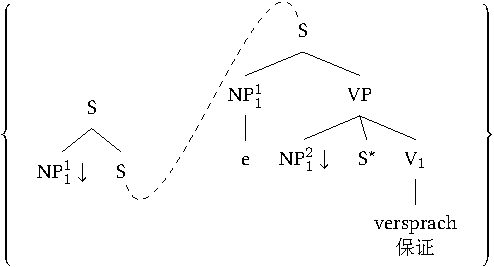
\includegraphics{Figures/tag-versprach-lsp-crop}
\caption{\label{Abbildung-MC-TAG-versprach}versprach的基本树集合包含了多元成分}
\end{figure}%
这棵树包括了一个被移动到左侧的NP$_1^1$的语迹,底部左侧的S结点和顶部右侧的S结点用虚线连接,表示支配关系。但我们并不要求直接支配关系,因此我们可以把这两棵子树分别插入到另外一棵树中,从而得到图\vref{Abbildung-TAG-Permutation3}中的语序。
\begin{figure}
\centerline{%
\begin{forest}
tag
[S
	[NP$_1^1\downarrow$]
	[S
		[NP$_2^2\downarrow$]
		[S
			[NP$_1^1$
				[e]]
			[VP
				[NP$_1^2\downarrow$]
				[S
					[NP$_2^1\downarrow$]
					[S
						[NP
							[PRO]]
						[VP
							[NP$_2^1$
								[e]]
							[NP$_2^2$
								[e]]
							[V$_2$
								[zu überführen;\textsc{inf} 起诉]]]]]
%								[zu überführen;to indict]]]]]
				[V$_1$
					[versprach;保证]]]]]]
%					[versprach;promised]]]]]]
\end{forest}
}
\caption{\label{Abbildung-TAG-Permutation3}针对语序NP$_1^1$ NP$_2^2$ NP$_1^2$ NP$_2^1$ V$_{2}$V$_{1}$的分析:附接操作作用于NP$_2^2$与NP$_2^1$之间的S结点}
\end{figure}%


\isc{多成分树邻接语法}\is{Multi-Component TAG}
\isc{树邻接语法(TAG)!多成分树邻接语法(MC-TAG)|)}\is{Tree Adjoining Grammar (TAG)!Multi"=Component (MC-TAG)|)} 
%Andere Varianten, die andere Konstituentenanordnungen zulassen sind V-TAG
其它允准上述结构成分语序的TAG变体包括V-TAG\isc{树邻接语法(TAG)!矢量树邻接语法(V-TAG)}\is{Tree Adjoining Grammar (TAG)!Vector (V-TAG)}\citep{Rambow94a}和TT-MC-TAG\citep{Lichte2007a}。\isc{树邻接语法(TAG)!树元组多成分树邻接语法(TT-MC-TAG)}\is{Tree Adjoining Grammar (TAG)!Tree Tuple MC-TAG (TT-MC-TAG)}\isc{成分序列|)}\is{constituent order|)}

\section{动词位置}

动词的位置
\isc{动词位置|(}\is{verb position|(}也可以做和GPSG并行的分析:在一个给定的序列线性化域(linearization domain)中,我们既可以让动词实现在前置位置上也可以实现在后置位置上。动词位置对小句的类型有影响,进而会影响到语义,基于词汇规则的分析同样可行:可以让一条词汇规则将一棵在后置位置放置了动词的树变成一棵在前置位置放置了定式动词的树。这和GB、最简方案以及HPSG的分析是相似的。 
\isc{动词位置|)}\is{verb position|)}

\section{被动}

类似转换生成语法中的转换机制,可以设计一种分析方法来处理被动
\isc{被动|(}\is{passive|(}:通过词汇规则来根据一个针对主动形式的词汇项,
来推出相应的被动形式基本树\citep[\page 50--51]{KJ85a},这里的主动形式的词汇项指那些包含了主动形式的相应基本树的词汇项。

\citet[\page 55]{KJ85a}提出了替代这种基于转换的分析的另一种方法,能够更好地处理被称之为“提升”
\isc{提升}\is{raising}的语言现象。他们的分析假定动词的论元都位列于子类框架(subcategorization)表中。如果一个动词匹配了某棵树相应的子类框架表,这个动词就可以进入到这棵树中。对应第\pageref{pass-lr-mlr}页讨论过的HPSG的词汇规则,Kroch和Joshi形式化得到了一条(TAG)词汇规则:该规则的输入端显式地提及一个宾格宾语。Kroch和Joshi针对非人称被动提出了一种复杂的分析,在不及物动词里没有实现出来的宾语,他们使用了语义上为空的角色来处理(第56页)。
这样的一种使用抽象的辅助实体的方式事实上是可以避免的:我们可以采纳始于\citet{Haider86}的HPSG\indexhpsgc 分析,我们在\ref{Abschnitt-HPSG-Passiv}中讨论过这种分析。

也有人提议
\isc{多重承继}\is{inheritance!multiple|(}使用承继关系来处理配价变化,被动仅仅被视为是一种特殊的配价变化现象(参见\citealp{Candito96a}及其扩展分析——\citealp*{KSYJ2006a})。正如我们在构式语法的相关讨论(见\ref{Abschnitt-Passiv-CxG})中所看到的,承继关系对于处理配价变化并不是理想的描写工具。这是因为这种处理手段在多个环节都存在句法和语义的交互(\citealp{Mueller2006d,Mueller2007d};\citeyear[\S~7.5.2]{MuellerLehrbuch1};\citeyear{MuellerUnifying};\citeyear{MWArgSt})。也请参见本书的\ref{relations-sec}了解更多的针对性讨论。 
\isc{多重承继}\is{inheritance!multiple|)}
\isc{被动|)}\is{passive|)}

\section{长距离依存}
\label{TAG-Fernabh}

\il{English|(}
\isc{长距离依存}\is{long"=distance dependency|(}TAG的长距离依存分析可以凭借其提供的标准工具——简单树可以插入到其它树的中间——进行分析。
图\vref{abb-nld-TAG}是(\mex{1})分析的一个实例:
\ea
\gll Who$_i$ did John tell Sam that Bill likes \_$_i$?\\
     谁 \textsc{aux} John 告诉 Sam \textsc{comp} Bill 喜欢 \\
\glt `John告诉Sam了,Bill喜欢谁?'
\z
%
\begin{figure}
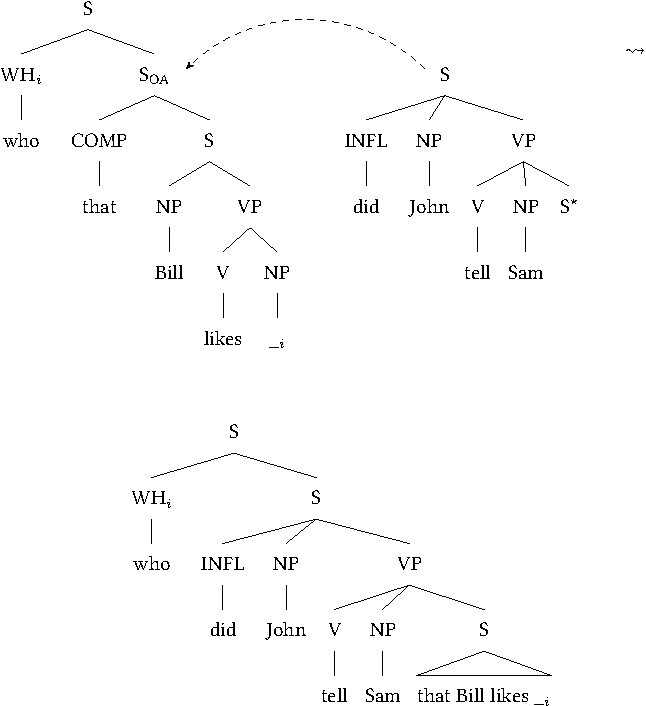
\includegraphics{Figures/tag-long-distance-dependencies-crop}
%%
%% Does not work with texlive 2015
%% %\oneline{%
%% \centerline{%
%% \begin{forest}
%% tag
%% [S
%% 	[WH$_i$
%% 		[who]]
%% 	[\tikzmark{soa}{S\sub{OA}}
%% 		[COMP
%% 			[that]]
%% 		[S
%% 			[NP
%% 				[Bill]]
%% 			[VP
%% 				[V
%% 					[likes]]
%% 				[NP
%% 					[\noexpand\_$_i$]]]]]]
%% \end{forest}
%% \hspace{0.5cm}
%% \begin{forest}
%% tag
%% [\tikzmark{s}{S}
%% 	[INFL
%% 		[did]]
%% 	[NP
%% 		[John]]
%% 	[VP
%% 		[V
%% 			[tell]]
%% 		[NP
%% 			[Sam]]
%% 		[S*]]]
%% \end{forest}
%% \qquad \raisebox{2cm}{$\rightsquigarrow$} \qquad
%% }\vspace{2\baselineskip}
%% \begin{forest}
%% tag
%% [S
%% 	[WH$_i$
%% 		[who]]
%% 	[S
%% 		[INFL
%% 			[did]]
%% 		[NP
%% 			[John]]
%% 		[VP
%% 			[V
%% 				[tell]]
%% 			[NP
%% 				[Sam]]
%% 			[S
%% 				[that Bill likes \noexpand\_$_i$, triangle]]]]]
%% \end{forest}
%% \begin{tikzpicture}[overlay,remember picture]
%% \draw[->, dashed, bend angle=45, bend right] ($(pic cs:s)+(-0.25,0.2)$) to($(pic cs:soa)+(0.8,.2)$);
%%
%% \end{tikzpicture}
%%
%% {%\dotted
%% % todo \anodecurve[l]{s4}[tr]{s2}{0.1in}[3ex]%
%% }
%% \hspace{1ex}
%% $\leadsto$
%}
\caption{\label{abb-nld-TAG}TAG中的长距离依存分析}
\end{figure}%
“WH COMP NP likes \_$_i$”的树属于likes的树族,因此包含在词典之中。
tell可以附接到这个树上,因为tell的这个树可以插入到“who that Bill likes \_$_i$”这棵树的中间位置。
这样一个插入性的操作可以重复很多次,所以在像(\mex{1})这样的句子中,who可以跨越多个小句边界移动到很远的位置:
\ea 
\gll Who$_i$ did John tell Sam that Mary said that Bill likes \_$_i$?\\
     谁      \textsc{aux} John 告诉 Sam \textsc{comp} Mary 说 \textsc{comp} Bill 喜欢\\
\glt `John告诉Sam,Mary说Bill喜欢谁?'
\z
%
还有一个很重要的细节:尽管(\mex{1})中的树包含范畴S,(\mex{1})并不是一个合语法的英语句子。
\ea[*]{
\gll who that Bill likes\\
谁 \textsc{comp} Bill 喜欢\\
}
\z
这一点必须通过TAG语法得到体现。在TAG中,额外OA符号可以用来标记一棵树的不完整性。如果一棵树包含了做了OA标识的结点,那么我们必须在这个结点处施加一次附接操作。
\isc{附接!附接的必要性|(}\is{adjunction!obligatory|(}
\il{English|)}
\isc{长距离依存|)}\is{long"=distance dependency|)} 

\section{新的发展和理论变体}

在\ref{Abschnitt-MC-TAG}中,我们介绍了多元成分TAG。事实上,存在很多不同的TAG变体,它们有着不同的形式性质。
\citet[\page]{Rambow94a}总结了截止到1994年的各种TAG变体。接下来,我将讨论两个有趣的TAG变体:基于特征结构的TAG(Feature Structure-based TAG,简称FTAG\indexftagc,\citealp{VSJ88a})和基于向量的TAG(Vector-based TAG,简称V"=TAG,\citealp{Rambow94a})。

\subsection{FTAG}

在FTAG
\isc{树邻接语法(TAG)!基于特征结构的树邻接语法(FTAG)|(}\is{Tree Adjoining Grammar (TAG)!Feature Structure"=Based (FTAG)|(}中,结点并不是原子的(N、NP、VP或S),而是包含有特征描写。
除了用于进行替换的结点之外,每一个结点都有一个顶结构、一个底结构。其中,顶结构说的是一棵树作为一个大的结构的一个子部分应该具有的属性,而底结构则陈述了某一个结点下面的成分应该具有的属性。用于替换的结点只有一个顶结构。图\vref{Abbildung-FTAG-laughs}是laughs(笑)的树结构实例。\todostefan{geschwungenen Pfeil, alignierte Knoten}
\begin{figure}
\centerline{%
\begin{forest}
tag
[{\ms{
   cat & {\upshape S}\\
 }\\
\ms{
   cat & {\upshape S}
}}
  [\ms{
    cat & {\upshape NP}\\
    agr & \ibox{1}\\
   }
%
   [{[~]\\
    \ms{
       cat & {\upshape NP}\\
       agr & \ms{
              per & 3\\ 
              num & sing\\
             }\\
      }}, substitution,tier=2
      [John;John, tier=word] ] ]
  [{\ms{
     cat & {\upshape VP}\\
     agr & \ibox{1} \ms{
                    per & 3\\ 
                    num & sing\\
                    }\\
     }\\
     \ms{ 
     cat & {\upshape VP}\\
     }}
     [{\ms{
          cat & {\upshape V}\\
         }\\
       \ms{
          cat & {\upshape V}\\
       }}, tier=2
       [laughs;笑,tier=word]]]
] 
\end{forest}
}
\caption{\label{Abbildung-FTAG-laughs}John和laughs在FTAG中的基本树}
\end{figure}%
一个名词短语可以和图\ref{Abbildung-FTAG-laughs}中的laughs的子树组合。它的顶结构需要和laughs树中的NP结点一致。
组合的结果如图\vref{Abbildung-FTAG-John-laughs}所示。
\begin{figure}
\centerline{%
\begin{forest}
tag
[{\ms{
   cat & {\upshape S}\\
 }\\
\ms{
   cat & {\upshape S}
}}
  [{\ms{
    cat & {\upshape NP}\\
    agr & \ibox{1}\\
   }\\
    \ms{
       cat & {\upshape NP}\\
       agr & \ms{
              per & 3\\ 
              num & sing\\
             }\\
      }}
      [John;John, tier=word] ]
  [{\ms{
     cat & {\upshape VP}\\
     agr & \ibox{1} \ms{
                    per & 3\\ 
                    num & sing\\
                    }\\
     }\\
     \ms{ 
     cat & {\upshape VP}\\
     }}
     [{\ms{
          cat & {\upshape V}\\
         }\\
       \ms{
          cat & {\upshape V}\\
       }}
       [laughs;笑,tier=word]]]
] 
\end{forest}
}
\caption{\label{Abbildung-FTAG-John-laughs}John树与laughs树在FTAG中的组合}
\end{figure}%

在一棵完整的树中,所有的顶结构都需要和其所对应的底结构一致。在这种组合方式下,只有主语为第三人称单数形式的句子才能使用所给定的laughs的子树,也就是说动词的一致性特征(agreement feature)必须和主语一致。

对于附接语来说,待插入成分的顶结构必须和附接树的顶结构合一,而底结构必须和附接树上的标有`*'的结点(所谓的底部结点(foot node)
\isc{底部结点}\is{foot node})的底结构合一。

目前所讨论的基本树只包含顶结构部分和底结构部分匹配的那些结点。FTAG允许一种特殊的变体,即某些结点可以声明在这些结点的位置必须进行附接操作,只有这样,其推导才是良形式(well-formed)的。
图\vref{Obl-Adjunktion-FTAG}展示了laughing的树,这棵树上的VP结点的两个结构中的\textsc{mode}特征的值不一致。
\begin{figure}
\centerline{%
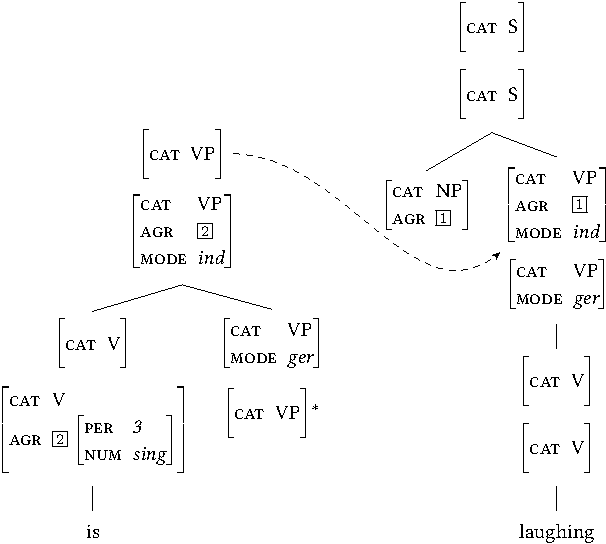
\includegraphics{Figures/tag-obl-adj-ftag-cropped}
}
% This does not work with texlive 2015 use texlive 2013
%% \hfill
%% \begin{forest}
%% [{\subnode{vpone}{\ms{
%%    cat & {\upshape VP}\\
%%  }}\vspace{2mm}\\ 
%%  \ms{
%%        cat & {\upshape VP}\\
%%        agr & \ibox{2}\\ 
%%        mode & ind\\
%%  }}
%%   [{\ms{
%%        cat & {\upshape V}\\
%%       }\vspace{2mm}\\
%%     \ms{
%%       cat & {\upshape V}\\
%%       agr & \ibox{2} \ms{
%%                       per & 3\\ 
%%                       num & sing\\
%%                      }\\
%%        }} [is]]
%%   [{\ms{
%%        cat & {\upshape VP}\\ 
%%        mode & ger\\
%%       }\vspace{2mm}\\
%%     \ms{
%%        cat & {\upshape VP}\\
%%        }$^*$}]]
%% \end{forest}
%% %% %%% sings tree:
%% %% \hspace{-1em}
%% \hfill
%% \begin{forest}
%% [{\ms{ 
%%    cat & {\upshape S}\\
%%  }\vspace{2mm}\\
%%  \ms{
%%   cat & {\upshape S}\\ 
%%   }}
%%   [\ms{ cat & {\upshape NP}\\
%%         agr & \ibox{1}\\
%%       }]
%%   [{\subnode{vptwo}{\ms{
%%       cat  & {\upshape VP}\\
%%       agr  & \ibox{1}\\
%%       mode & ind\\
%%       }}\vspace{2mm}\\
%%      \ms{
%%      cat & {\upshape VP}\\ 
%%      mode & ger\\
%%      }}
%%      [{\ms{ cat & {\upshape V}\\
%%           }\vspace{2mm}\\
%%        \ms{
%%             cat & {\upshape V}\\
%%         }}
%%        [laughing]]]]
%% \end{forest}
%% \hfill\mbox{}
%% \begin{tikzpicture}[overlay,remember picture,out=0,in=220]
%% \draw[->, dashed] (vpone) to (vptwo);
%% \end{tikzpicture}
\caption{\label{Obl-Adjunktion-FTAG}FTAG中的强制附接}
\end{figure}%
为了将这棵树组成一个完整结构,必须添加另外一棵树以便将VP结点的两个部分分隔开来。这需要借助一棵附接树(如图\ref{Obl-Adjunktion-FTAG}中的附接树)来实现。附接树的最高位置的VP结点和laughing中VP结点,二者各自的顶结构需要合一。附接树中标有`*'号的结点和laughing中VP结点,二者的底结构合一。其结果如图\vref{Obl-Adjunktion-FTAG-Ergebnis}所示。
\begin{figure}
%%% is laughing tree:
\centerline{%
\begin{forest}
[{\ms{ 
   cat & {\upshape S}\\
 }\vspace{1mm}\\
  \ms{
   cat & {\upshape S}\\
  }}
  [{\ms{ cat & {\upshape NP}\\
         agr & \ibox{1}\\
   }}]
  [{\ms{
     cat  & {\upshape VP}\\
     agr  & \ibox{1}\\
     mode & ind\\
    }\vspace{1mm}\\
    \ms{
       cat & {\upshape VP}\\
       agr & \ibox{2}\\ 
       mode & ind\\
    }}
    [{\ms{
       cat & {\upshape V}\\
      }\vspace{1mm}\\
      \ms{
        cat & {\upshape V}\\
        agr & \ibox{2} \ms{
                per & 3\\ 
                num & sing\\
               }\\
         }} [is\\\textsc{aux}]]
     [{\ms{
        cat & {\upshape VP}\\ 
        mode & ger\\
      }\vspace{1mm}\\
      \ms{
       cat & {\upshape VP}\\ 
       mode & ger\\
      }}
      [{\ms{ cat & {\upshape V}\\
           }\vspace{1mm}\\
        \ms{
             cat & {\upshape V}\\
        }} [laughing\\笑]]]]]
\end{forest}
}
  \caption{\label{Obl-Adjunktion-FTAG-Ergebnis}FTAG中强制附接的结果}
\end{figure}%

推导到最后所得到的那棵树,需要将所有结点各自的顶结构与底结构进行合一。图\ref{Obl-Adjunktion-FTAG-Ergebnis}中树的最高的VP结点的顶结构和底结构的\textsc{agr}特征值需要合一。正因为这个原因,只有和附接树中的\textsc{agr}特征取值一样的NP树才能插入当前树中的NP槽中。
%此处只能意义,原文若探究字面意义,不仅不通顺,还算是写错了。

这个例子展示了,我们在处理长距离依存时曾经采用过的强制附接
\isc{附接!附接的必要性}\is{adjunction!obligatory}机制可以通过令顶结构和底结构特征取值不一致来实现。
如果一棵树中存在不兼容的顶结构与底结构,这棵树就不能是最终的导出树。%又一个错误
这意味着至少需要再进行一次附接操作才能得到良形式的树。
\isc{树邻接语法(TAG)!基于特征结构的树邻接语法(FTAG)|)}\is{Tree Adjoining Grammar (TAG)!Feature Structure"=Based (FTAG)|)}

\subsection{V"=TAG}
\label{sec-vtag}

V"=TAG
\isc{树邻接语法(TAG)!矢量树邻接语法(V-TAG)|(}\is{Tree Adjoining Grammar (TAG)!Vector (V-TAG)|(}是Owen\citet{Rambow94a}提出来的一种TAG变体,它同样包含了特征结构。
除此之外,和MC"=TAG一样,它假定以基本树的集合作为分析单元。图\vref{Abbildung-Lexical-Set-geben-V-TAG}是双宾动词geben(给)的基本词汇描写。
\begin{figure}
\vspace{4\baselineskip}
\menge{ 
\forestset{begin draw/.code={\begin{tikzpicture}[baseline=(current bounding box.center)]}}
    \hspace{1em}
    \begin{forest}
    [, phantom, for children={if n'=1{before computing xy={s*=1.25}}{}}
       %% This adjusts the relative position of the last child by zeroing its distance from the
       %% phantom root and increasing its distance from its sibling. This is delayed because 
       %% otherwise Forest will undo any changes when packing the tree.
      [VP
            [NP$\downarrow$]
            [VP, tikz+={\ignoreme\draw [densely dashed] ([yshift=2.5pt].south) [out=-75, in=-125] to ($(!u.north)!3/4!(!un.north)$) [out=55,in=100] to (!rl.north); }]]
    [VP
            [NP$\downarrow$]
            [VP, tikz+={\ignoreme\draw [densely dashed] ([yshift=2.5pt].south) [out=-75, in=-125] to ($(!u.north)!3/4!(!un.north)$) [out=55,in=100] to (!rl.north); }]]
    [VP
            [NP$\downarrow$]
            [VP, tikz+={\ignoreme\draw [densely dashed] ([yshift=2.5pt].south) [out=-75, in=-125] to ($(!u.north)!3/4!(!un.north)$) [out=55,in=100] to (!rl.north); }]]
    [VP
            [geben\\给]
%             [geben]
            [VP, tikz+={\ignoreme\draw [densely dashed] ([yshift=2.5pt].south) [out=-75, in=-125] to ($(!u.north)!3/4!(!un.north)$) [out=55,in=100] to (!rl.north); }]]
    [VP
            [$\epsilon$]]]
    \end{forest}
    \hspace{1em}
}
\vspace{.4\baselineskip}
  \caption{\label{Abbildung-Lexical-Set-geben-V-TAG}
    遵照\citet[\page 6]{Rambow94a}的geben(给)在V"=TAG中的词汇描写
  }
\end{figure}%
这个词汇描写包括了给定动词的一棵树,一个范畴为VP的空成分,三棵用于将VP和NP结合起来的树。像MC"=TAG一样,对支配关系进行了显性声明。
图\ref{Abbildung-Lexical-Set-geben-V-TAG}中的支配限制要求每棵树中位于低处的VP结点都支配了最右侧的树的最高处的VP结点。动词论元的顺序以及动词的位置并没有给定。唯一限定的是:带有NP的树的低处的VP,以及geben(给)的低处的VP要支配空成分的VP。有了这一树集合,我们可以推出论元顺序的任意一种排列。Rambow同时也展示了如何利用词汇项来分析动词复合体。图\vref{Abbildung-zu-reparieren-versprochen-V-TAG}展示了由“zu reparieren”(修补)和versprochen(保证)组成的动词复合体的树集描写,其中包含了支配关系限制。
\begin{figure}
\vspace{4\baselineskip}
\oneline{%
\menge{%
  \begin{forest}
    [, phantom, for children={if n'=1{before computing xy={l=0pt, s*=1.25}}{}}
       %% This adjusts the relative position of the last child (n'=1) by zeroing its distance from the
       %% phantom root (l=0) and increasing its distance from its sibling. This is delayed because 
       %% otherwise Forest will undo any changes when packing the tree.
      [VP
        [NP$\downarrow$]
        [VP, tikz+={\ignoreme\draw [densely dashed] ([yshift=2.5pt].south) [out=-75, in=-125] to
            ($(!u.north)!3/4!(!un.north)$) %[out=55,in=181]  to ++(4cm,2cm) [out=-1,in=90] 
            [out=55,in=90] to (!rll.north); }]
        % the following line is ignored for space computation due to \ignoreme
        % the first VP node at the baseline is connected to a place between the dominating vp !u.north and the node to the
        % left of it !un.north (the second VP node on the second line). 3/4 specifies the position
        % between these nodes. It is more to the second VP. From there we go to rll, which is the
        % root node's (r) last child's (l) last child (l). Since the root node is our phantom node,
        % the rll node is the last VP in the second row.
        %
        % the yshift raises the beginning of the line so that it is not too far away from the node.
      ]
      [VP
        [NP$\downarrow$]
        [VP, tikz+={\draw [densely dashed] ([yshift=2.5pt].south) [out=-80, in=180] to ++(20mm,-15mm) [out=0, in=-90] to ($(!unn.north)!.7!(!unnn1.north)$) [out=90, in=180] to ++(3.5mm,5mm) [out=0, in=90] to (!rl1.north); }]
      ]
      [VP
        [NP$\downarrow$]
        [VP, tikz+={\draw [densely dashed] ([yshift=2.5pt].south) [out=-80, in=180] to ++(10mm,-10mm) [out=0, in=-90] to ($(!un.north)!.6!(!unn1.north)$) [out=90, in=180] to ++(5.5mm,6.5mm) [out=0, in=90] to (!rl1.north); }]
      ]
      [VP
        [NP$\downarrow$]
        [VP, tikz+={\draw [densely dashed] ([yshift=2.5pt].south) [out=-80, in=-105] to ($(!u.north)!1/3!(!un.north)$) [out=75,in=90] to (!rll.north); }]
      ]
      [VP
        [VP
          [$\epsilon$]
          [zu reparieren\\\textsc{inf} 修补]
%          [zu reparieren]
                  ]
        [VP, baseline
          [$\epsilon$]
          [versprochen\\保证]
%          [versprochen]
        ]
      ]
    ]
  \end{forest}
}
}
\vspace{2.5\baselineskip}
  \caption{\label{Abbildung-zu-reparieren-versprochen-V-TAG}V"=TAG中的动词复合体“zu reparieren versprochen”的分析}
\end{figure}%%
其中的两棵带有NP的树支配了versprochen,而另外两棵支配了zu reparieren。
带有NP的树的次序并没有被限制,因而这些NP间的任意排列都是被允准的。\pagebreak

这个地方有意思的是这种方法和\citet[\S~2.1.3]{Berman96a-u}在LFG\indexlfgc 中的分析很像(参见\ref{Abschnitt-LFG-Umstellung}):
在Berman的分析中,动词直接投射(project)并形成VP,然后附接上论元。

和本书中讨论的其它分析不同的是:不管动词位置如何,导出树中总是有一个空成分。
\isc{空成分}\is{empty element} 
\isc{树邻接语法(TAG)!矢量树邻接语法(V-TAG)|)}\is{Tree Adjoining Grammar (TAG)!Vector (V-TAG)|)}

\subsection{语言能力与语言运用的区分以及树本地化的MC"=LTAG的生成能力}
%\subsection{The competence"=performance distinction and the generative capacity of tree"=local MC"=LTAG}
\label{Abschnitt-Kompetenz-Performanz-TAG}

本书中
\isc{语言能力|(}\is{competence|(}
\isc{语言运用|(}\is{performance|(}讨论的很多理论都区分语言能力(competence)和语言运用(performance)\citep[\S~I.1]{Chomsky65a}。我们假定语言能力理论描写语言知识,而语言运用理论应该解释语言知识如何被使用以及为什么我们在使用和理解语言的过程中会产生错误等问题。参见\S \ref{chap-competence-performance}了解更多的讨论。 

\citet*{JBR2000a}讨论了如(\mex{1}b)所示的关系从句的中心自嵌入问题(center self embedding),他们遵循\citet[\page 286]{CM63a}的假定:这种嵌入最多只可能有三级的这一事实不应该在语法中进行描写,而应该归属于听者的加工问题,而这与语法的描写能力无关。
\eal
\label{TAG-Beispiel-Performanz}
\ex 
\gll dass der Hund bellt, der  die Katze jagt,  die  die Maus  gefangen hat\\
%    that the dog  barks  that the cat   chases that the mouse caught   has\\
%\glt `that the dog that chases the cat that caught the mouse barks'
     \textsc{comp} \textsc{det} 狗  叫  \textsc{rel} \textsc{det} 猫 追 \textsc{rel} \textsc{det} 老鼠 捉 \textsc{aux}   \\
\glt `追着那只捉老鼠的猫的那只狗在叫'
\ex 
\gll dass der Hund, [$_1$ der  die Katze, [$_2$ die  die Maus  gefangen hat,~$_2$] jagt~$_1$] bellt\\
     %that the dog   {}    that the cat    {}    that the mouse caught   has        chases    barks\\
     \textsc{comp} \textsc{det} 狗  {}  \textsc{rel} \textsc{det} 猫 {} \textsc{rel} \textsc{det} 老鼠 捉 \textsc{aux}   捉 叫 \\
\glt `追着那只捉老鼠的猫的那只狗在叫'
\zl

\noindent
这里有意思的是可以构建对于听者来说更为简单的中心嵌入(center embedding)的例子。基于这样的方式,我们可以构建一些可以被加工处理的数量更多的中心嵌入的例子,从而说明了严格假定关系从句最多只能做两级中心嵌入的语法是错误的。以下是Hans Uszkoreit\aimention{Hans Uszkoreit}举的例子,它更容易被加工,因为所有的嵌入的关系从句都被隔离开来并且动词和更高层的小句也被隔离了。
\ea
\gll Die Bänke, [$_1$ auf denen damals die Alten des Dorfes, [$_2$ die allen Kindern, [$_3$~die vorbeikamen $_3$], freundliche Blicke zuwarfen $_2$], 
lange Stunden schweigend nebeneinander saßen $_1$], mussten im letzten Jahr einem~~~~~~~ Parkplatz weichen.\\
\textsc{det} 长椅 {} \textsc{prep} 那 当时 \textsc{det} 老.人 \textsc{det} 村庄 {} \textsc{rel} 所有 儿童 \hspaceThis{[$_3$~}\textsc{rel} 经过 {} 友好地 目光 给 {}
长 小时 安静 彼此相邻 坐 {} 必须 \textsc{prep}.\textsc{det} 上一个 年 一 停车场 让道\\
%the benches {} on which back.then the old.people of.the village {} that all children {} that came.by {} friendly glances gave {}
%long hours silent next.to.each.other sat {} must in.the last year a car.park give.way.to\\
\glt `村子里的那些本来安静地彼此相邻的、供老居民们互相友好地照看所有经过的孩子的长椅们在去年不得不给停车场让道了。'
%\glt `The benches on which the older residents of the village, who used to give friendly glances to all the children who came by, used to sit silently next %to one another had to give way to a car park last year.'
\z
参见\citew{Gibson98a}了解其它的会影响语言加工的因素。

\citet{JBR2000a}讨论了动词复合体中的论元语序重列问题。他们所关注的模式如(\mex{1})所示:
\ea
$\sigma$(NP$_1$ NP$_2$ \ldots{} NP$_n$) V$_{n}$V$_{n-1}$ \ldots{} V$_{1}$
\z
这里,$\sigma$表示名词短语的任意一种排列,而V$_{1}$是定式动词。作者们探寻了与上述模式相关的词汇化树邻接语法(Lexicalized Tree Adjoining Grammar,简称LTAG)的性质,并注意到如果在考虑语义的情况下LTAG不能够分析这种语序。
\ea
NP$_2$ NP$_3$ NP$_1$ V$_{3}$V$_{2}$V$_{1}$
\z
因为在德语中,(\mex{1})是被允准的语言使用,因此LTAG并不足以描写任意语言。
\ea
\gll dass ihm$_2$ das Buch$_3$ niemand$_1$ zu lesen$_3$ versprechen$_2$ darf$_1$\\
%     that him     the book     nobody     to read      promise         be.allowed.to\\
%\glt `that nobody is allowed to promise him to read the book' 
     \textsc{comp} 他     \textsc{det} 书 没有人 \textsc{inf} 读 保证 被允许 \\
\glt `没有人被允许保证他读那本书'
\z
因此,他们提出扩展TAG,即所谓的树本地化多元成分LTAG(tree"=local multi"=component LTAG,简称为树本地化MC"=LTAG,或TL-MCTAG),参见\ref{Abschnitt-MC-TAG}的讨论。他们证明了基于正确的语义,TL-MCTAG可以分析(\mex{0})但不能分析(\mex{1})。他们声称在德语中不能出现这些语序,并且论证说在这种例子里,不像关系从句里的例子,我们可以有两种选择(也就是说,否定这种模式或基于语言运用或基于语言能力进行解释)。
\ea
\label{ex-mc-ltag-fails}
NP$_2$ NP$_4$ NP$_3$ NP$_1$ V$_{4}$V$_{3}$V$_{2}$V$_{1}$
\z
如果我们视之为语言运用现象,则我们参考的是构造过程的复杂度以及随之而来的听者的加工问题。根据协同性(cooperativeness)
\isc{合作性}\is{cooperativeness}原则来解释为何语料中没有出现过这些语序?说话者通常希望自己被理解,因此会尽量按照听者可以理解的方式来明确表达出他们的句子。德语中的包含超过四个动词的动词复合体很少见,因为可以通过外置(extraposing)
\isc{外置}\is{extraposition}操作来简化句子右侧有多个动词的复杂句子,从而避免歧义\citealp[\page 262]{MuellerLehrbuch1})。

而另一种不同于语言运用解释的分析则使用具有更强能力的语法理论,这样的语法理论一方面允许两个动词的嵌入以及对它们的论元进行重排序,另一方面排除三个动词的嵌入与论元重排序。\citet{JBR2000a}选择了这个解决方案,因此把(\mex{0})中所示语序的不合理性归结于语言能力。 

在HPSG(以及范畴语法\indexcgc 和一些GB分析\indexgbc)中,动词复合体通过论元组合进行解释\citep{HN89b,HN94a}。 在这种方法中,一个动词复合体的属性和一个简单动词完全一样,而所涉及到的动词的论元可以任意排列。语法并不限制用于组合的动词的数量,也不要求在一定层级之下禁止嵌入。接下来,我将论证许多种语序重列都是被交际规则排除掉的,这些交际规则甚至可以应用到只有两个动词的简单情况中。结论是无法嵌入四个或者更多的动词应该作为语言运用问题进行解释。

在介绍不同于基于语言能力去排除(\ref{ex-mc-ltag-fails})的观点之前, 我将提出一个更具一般性的观点:
在这里语料无法帮助我们,因为没有谁找到了嵌入四个以及更多动词的实例。\citet{Bech55a}提供了一个大量的实例集,但没有构造出任何包括四个嵌入动词的实例。\citet[\page 94--95]{Meurers99c}给了一些造出来的嵌入五个动词的例子,这五个动词中包含多个助动词和情态词。
这些例子都很难被加工,也和我们这里的讨论没有关系,因为(\ref{ex-mc-ltag-fails})中的动词必须选择它们自己的论元。
因此就构造例子而言并没有那么多的可供选择动词。可以仅仅使用带有一个额外宾语的主语控制(subject control)动词(如versprechen(保证))、宾语控制动词或AcI动词(如sehen(看)和lassen(听))来构造例子。
在构造例子的过程中,很重要的是确保所有涉及到的名词尽量采用不同的格
\isc{格}\is{case}和选择限制(selectional restrictions)
\isc{选择限制}\is{selection!restriction}(如有生命/无生命),因为一个听者/读者可以用这些特征来将语序重列的论元匹配到它们的中心词上。
如果我们希望有(\ref{ex-mc-ltag-fails})中的那种四个NP带有不同格的例子,那么我们必须选择一个支配属格的动词。
德语中只有很少几个这样的动词。尽管\citet{JBR2000a}在(\ref{Beispiel-Joshi-NP4})中构造的例子满足了这些要求,这仍然过于异常。
想在新闻文本中找到这样的例子,可能性极低,这一点十分清楚。这可能是因为只有很罕见的一些情境中,才能联想到这样的话语。
更进一步说,所有的控制动词(除了helfen(帮助))都需要一个带有zu的不定式,
并且也可以以内在并不一致的方式实现出来,也就是说通过包含一个外置的不定式附接语去除动词复合体。
我们已经提到过,一个有合作精神的说话者/写者愿意用一个不那么复杂的构式,而这将进一步降低这种句子出现的可能性。

请注意,TL-MCLTAG并不限制一个句子中能出现多少个动词。这套理论本身允许任意多的动词。因此我们需要像其他语法理论一样需要在语言运用的限制上做假设,以此解释为何我们完全找不到带有五个甚至更多个动词的动词复合体。TL-MCLTAG可以预测进行论元语序重列的可能性。
我认为依赖语法形式模型的表达能力来对论元移位情况进行限制是不合理的,因为这些限制独立于动词复合体而存在,这些限制同样也可以在只包括两个论元的简单动词中出现。语序重列的问题在于仍然有可能将名词短语分配给它们所属的动词。如果这个分配导致歧义
\isc{歧义}\is{ambiguity},并且这种歧义无法通过格、选择限制、上下文知识或语调消解,则会选择无标记的成分语序。
\citet*[\page 68]{Hoberg81a}论证了基于这一点可以很好地处理诸如下面实例的语言现象\footnote{%
Hoberg使用的是代词的所有格——ihr(她),而不是das(\textsc{det})。
这使得句子语义上更加通顺,但被约束的代词的序列线性化的要求可能干预相应的句法过程。因此,在这里我将代词换成了定冠词。
}:
\eal
\judgewidth{\#}
\ex[]{
\gll Hanna hat immer schon gewußt, daß das Kind sie verlassen will.\\
%	 Hanna has always already known that the child she leave wants\\
%\glt `Hanna has always known that the child wants to leave her.'
	 Hanna \textsc{aux} 总是 已经 知道 \textsc{comp} \textsc{det} 孩子 她 离开 希望 \\ 
\glt `Hanna一直都知道孩子希望离开她。'
}
\ex[\#]{
\gll Hanna hat immer schon gewußt, daß sie das Kind verlassen will.\\
%     Hanna has always already known that she the child  leave wants\\
%\glt Preferred reading: `Hanna has always known that she wants to leave the child.'
      Hanna \textsc{aux} 总是 已经 知道 \textsc{comp} 她 \textsc{det} 孩子 离开 希望 \\ 
\glt 倾向于解读为:`Hanna一直都知道她希望离开孩子。' 
}
\ex[]{
%\raggedright
\gll Hanna hat immer schon gewußt, daß sie der Mann verlassen will.\\
%     Hanna has always already known that she the.\nom{} man leave wants.to\\
     Hanna \textsc{aux} 总是 已经 知道 \textsc{comp} 她 \textsc{det}.\nom{} 男人 离开 希望\\\hspace{-4pt}
\glt `Hanna一直都知道那个男人希望离开她。' 
%\glt `Hanna has always known that the man wants to leave her.'
}
\zl

\noindent
除非是对另外一种解读有很强的倾向性,否则不太可能将例(\mex{0}a)的语序换成例(\mex{0}b)中的语序。
这是因为无论sie(她)还是“das Kind”(孩子)都没有被无歧义地标示成主格或者宾格。(\mex{0}b)因此必须解读为Hanna是那个想要离开孩子的那个人。当然,如果至少一个论元被无歧义地做了格标记,这个语序重列也是可能的,就像例(\mex{0}c)那样。

对于由阴性可数名词组成的名词短语来说,主格和宾格的形式,属格和与格的形式相同。
对于不可数名词,情况更加糟糕。如果它们不加冠词,阴性名词的所有的格形式都是一样的,例如Milch(牛奶)。
阳性和中性词的属格也有类似之处。在下面\citet[\page 45]{Wegener85b}的例子中,很难交换与事与宾格宾语的位置,而当名词像(\mex{1}c、d)样配有冠词时则可以做这种交换。

\eal
\ex 
\gll Sie mischt Wein Wasser bei.\\
%     she mixes wine water into\\
%\glt `She mixes water into the wine.'
     她 混合 酒 水 \textsc{prep} \\
\glt `她将水混到酒里。'
\ex 
\gll Sie mischt Wasser Wein bei.\\
%     she mixes water wine into\\
%\glt `She mixes wine into the water.'
     她 混合 水 酒 \textsc{prep} \\
\glt `她将酒混到水里。'
\ex 
\gll Sie mischt dem Wein das Wasser bei.\\
%     she mixes the.\dat{} wine the.\acc{} water into\\
%\glt `She mixes the water into the wine.'
     她 混合 \textsc{det}.\dat{} 酒 \textsc{det}.\acc{} 水 \textsc{prep} \\ 
\glt `她将水混到酒里。'
\ex 
\gll Sie mischt das Wasser dem Wein bei.\\
%    she mixes the.\acc{} water the.\dat{} wine into\\
     她 混合 \textsc{det}.\acc{} 水 \textsc{det}.\dat{} 酒 \textsc{prep} \\ 
%\glt `She mixes the water into the wine.'
\glt `她将水混到酒里。'
\zl
如果句子的意义在上下文中是清楚的(例如通过显性的否定),或者句子带有明确的语调,那么两个动词可以交换。

动词复合体的问题是:如果我们不希望通过限制更少的动词支配所有格的话,四个名词短语中有两个几乎一直会有一样的格。
(\mex{1})是一个听起来有点别扭的例子,它通过形态变化来无歧义地标记了格:
\ea
\gll weil    er        den        Mann dem        Jungen des Freundes gedenken helfen lassen will\\
%     because he.\nom{} the.\acc{} man  the.\dat{} boy    of.the.\gen{} friend remember help let wants\\
%\glt `because he wants to let the man help the boy remember his friend'
     因为 他.\nom{} \textsc{det}.\acc{} 男人  \textsc{det}.\dat{} 男孩    \textsc{det}.\gen{} 朋友 记得 帮助 让 希望 \\
\glt `因为他希望让那个男人帮助那个男孩记得他的朋友' 
\z
另一个策略是控制动词对有生和无生宾语的选择,通过论元的有生性来辅助解释。
我构造了一个例子,在这个例子中,在深层位置嵌入的谓词是一个形容词而非动词。谓语leer fischen(钓光了)是一个结果构式,这个构式需要和动词复合体进行类比分析\citep[\S~5]{Mueller2002b}。
\ea
\gll weil niemand$_1$ [den Mann]$_2$ [der Frau]$_3$ [diesen Teich]$_4$  leer$_4$ fischen$_3$ helfen$_2$ sah$_1$\\
%     because nobody.\nom{} \spacebr{}the.\acc{} man \spacebr{}the.\dat{} woman \spacebr{}this.\acc{} pond empty fish help saw\\
     因为 没有人.\nom{} \spacebr{}\textsc{det}.\acc{} 男人 \spacebr{}\textsc{det}.\dat{} 女人 \spacebr{}这个.\acc{} 池塘 空 钓鱼 帮助 看见 \\
%\glt `because nobody saw the man help the woman fish the pond empty'
\glt `因为没有人看见那个男人帮助那个女人把池塘里的鱼钓光了' 
\z
阅读句子的时候带有相应的停顿可以使得句子的意义得到理解。有生的名词短语格可以被无歧义地标记格,我们的词汇知识可以帮助我们将diesen Teich(这个池塘)解释为leer(空)的论元。 

(\mex{0})中的句子可以通过一个适当的TL-MCLTAG进行分析,也可以通过动词复合体或结果构式的论元组合进行分析。(\mex{1})中的句子是对应于(\ref{ex-mc-ltag-fails})的模式并且类似(\mex{0})的例子:
\ea
\gll weil [der Frau]$_2$ [diesen Teich]$_4$ [den Mann]$_3$ niemand$_1$ leer$_4$ fischen$_3$ helfen$_2$ sah$_1$\\
% because \spacebr{}the.\dat{} woman \spacebr{}this.\acc{} pond \spacebr{}the.\acc{} man nobody.\nom{} empty fish help saw\\
  因为 \spacebr{}\textsc{det}.\dat{} 女人 \spacebr{}这个.\acc{} 池塘 \spacebr{}\textsc{det}.\acc{} 男人 没有人.\nom{} 空 钓鱼 帮助 看见 \\
\glt `因为没有人看见那个男人帮助那个女人把池塘里的鱼钓光了'
\z
(\mex{0})比(\mex{-1})的形式标记更多,不过总是针对局部重列的现象(Gisbert Fanselow\aimention{Gisbert Fanselow}, p.\,c.\ 2006)。
这个句子不应该被语法排除掉。导致这些标记的因素和简单动词论元的标记性是一样的。TL-MCLTAG无法正确地分析诸如(\mex{0})中的例子,这说明这种TAG变体并不适合分析自然语言。

什么应该被视为语言能力?什么应该被视为语言运用?不同的TAG研究者有不同的意见。如\citet[\page 15]{Rambow94a}论证认为我们不应该排除那些语法或语法形式模型无法处理的语序重列。在第六章,他提出一个语言应用的理论,解释了为什么位于中间位置的动词的论元的语序重列问题比较难以处理。因此,我们应该选择像V-TAG
\isc{树邻接语法(TAG)!矢量树邻接语法(V-TAG)}\is{Tree Adjoining Grammar (TAG)!Vector (V-TAG)}或TT-MC-TAG
\isc{树邻接语法(TAG)!树元组多成分树邻接语法(TT-MC-TAG)}\is{Tree Adjoining Grammar (TAG)!Tree Tuple MC-TAG (TT-MC-TAG)}这样的TAG变体\citep{Lichte2007a},这些变体能够解释多种语序,然后可以使用语言运用模型来解释为什么句子可接受程度不同。

另一种寻找拥有最小表达能力的语法形式模型的思路是根本就不去限制形式模型的表达能力,而是去尽量限制语言学理论本身。在第\ref{sec-generative-capacity}章中,我们将展开更多的讨论。 
\isc{语言能力|)}\is{competence|)}
\isc{语言运用|)}\is{performance|)}

\section{总结与分类}

总的来说,LTAG是词汇化的理论,也就是说每棵树上都至少有一个词汇元素;没有树会对应像S $\to$ NP VP这样的规则,因为在这条规则中没有词出现。总有包含主语NP和VP的复杂的树。在VP内部会有必须的足够多的结构来确保树中包含动词。LTAG中的基本树总是包含中心词及其论元。对于及物动词,这意味着主语和宾语都必须成为基本树的成分。对于用于长距离依存分析的树,这也同样适用。正如图\ref{abb-nld-TAG}所示,宾语必须是树的一部分。宾语可以和动词之间可以间隔多个句子边界,这一点并没有在基本树中体现,也就是说,语法的递归性并没有在基本树中体现。相应的作用是通过附接操作来实现的,附接是指向树中间插入成分。用于抽取的基本树,如图\ref{abb-nld-TAG}所示,不同于用于解释普通SVO小句的基本树,如图\ref{Abbildung-Max-likes-Anouk}中的likes的基本树。 伴随likes的最小结构(如主语抽取、话题化、主语关系从句、宾语关系从句、被动等等)需要它们自己各自的基本树\citep[\page 10]{KJ2003a}。不同的基本树通过词汇规则
\isc{词汇规则}\is{lexical rule}联系在一起。这些词汇规则将一棵特定的树影射为其它的树。通过这种方式,可以从一个表示主动形式的树推出表示被动形式的树。这些词汇规则可以和转换语法中的转换规则
\isc{转换}\is{transformation}进行类比。 但必须强调一点,每个树中都有词汇元素,这使得整个语法和自由的转换相比更加受限。

和GB以及含有空成分的LFG、CG、HPSG变体的一个有意思的不同之处是这里介绍的TAG变体\footnote{%
  参见\citew{Rambow94a}和\citew[\page 194]{Kallmeyer2005a-u},以了解词典中带有空成分的TAG分析。
},其词典中并不包含空成分。空成分可以出现在树中,树再作为一个整体出现在词典中。

基本树的大小不受限制,这使得TAG在分析习语的时候特别方便(见第\ref{Abschnitt-Diskussion-Lokalitaet}节)。
因为递归从基本树中排除掉了,因此在导出树中距离特别远的元素可以包含在同一个基本树中(扩展的局域性\isc{定域}\is{locality})。

\citet*{KKNV95a}论证了满足特定要求的HPSG语法可以转写为TAG语法。通过这种方式,我们可以得到一个计算复杂度
\isc{生成能力}\is{capacity!generative}更明确的语法。HPSG语法一般都是0-型文法,而不同的TAG变体可以用来刻画从2-型语言到弱上下文相关语言
\isc{弱上下文相关语言}\is{mildly context"=sensitive grammar}之间的不同语言\citep{Joshi85a-u}。\citet*{YMTT2001a}提出了一个算法可以将FB"=LTAG语法翻译成弱上下文相关语言的HPSG文法。

%\section*{思考题}
\bigskip
\questions{
\begin{enumerate}
\item TAG是如何分析长距离依存的?在分析长距离依存的时候是否需要空成分?
\item 是否有可能通过标准的TAG过程来分析多个动词的论元的语序重列问题?
\end{enumerate} 
}

%\section*{练习题}
\exercises{
\begin{enumerate}
\item 用LTAG分析下列词串:
\ea
\gll der dem König treue Diener\\
% the the.\dat{} king loyal servant\\
  \textsc{det} \textsc{det}.\dat{} 国王 皇家 雇工\\
\glt `国王的皇家雇工'
\z
\end{enumerate}
}

%\section*{延伸阅读}
\furtherreading{
重要的论文包括\citew*{JLT75a-u}、\citew{Joshi87a-u}和\citew{JS97a}。很多更关心语言本体的读者并不会过多涉猎讨论TAG形式性质的论文。
\citew{KJ85a}很好地总结了针对语言现象的分析。 针对TAG的语言学与计算语言学的论文可以在Abeill{\'e}和Rambow\nocite{AR2000a-ed-not-crossreferenced}所编辑的论文中找到。\citet{Rambow94a}比较了他的TAG变体(V"=TAG
\isc{树邻接语法(TAG)!矢量树邻接语法(V-TAG)}\is{Tree Adjoining Grammar (TAG)!Vector (V-TAG)})和Karttunen的激进词汇主义(Radical Lexicalism)方法、Uszkoreit的GPSG\indexgpsgc、组合范畴语法\indexcgc, HPSG\indexhpsgc 以及依存语法\indexdgc。 

\citet{SJ93a}讨论了从心理语言学来说可行的加工模型,并且论证了基于TAG进行增量式句法分析的可行性。他们进一步提出了TAG的一种变体:同步TAG(synchronous TAG\indexstagc)。在这种TAG变体中,一棵句法树有一棵语义树与之相对应。当构建句法结构的时候,语义结构也同步构建起来。这个同步构建的结构对应于GB理论中通过转换
\isc{转换}\is{transformation}从表层结构中经由推导得到的逻辑形式(Logical Form
\isc{逻辑形式(LF)}\is{Logical Form (LF)})。

\citet[\S~6]{Rambow94a}展示了一个基于自动机的语言运用理论。他将这种理论应用到德语上并表示可以解释在对多个动词的论元进行重列加工时所遇到的困难。 
\isc{树邻接语法(TAG)|)}\is{Tree Adjoining Grammar (TAG)|)}

\citet{KR2008a-u}基于FTAG展示了如何通过一棵推导树进行MRS的获取。每一个顶结点都引用了整个结构的语义内容,而每一个底结点都引用了所在结点之下的部分的语义内容。基于这种方式,当把形容词(如mutmaßlichen(被怀疑的))插入到NP树(如alle Mörder(全部凶手))时,可以确保形容词有超过名词性部分(Mörder(凶手))的作用域:当把形容词附接到N结点时,形容词可以获取名词的语义内容。mutmaßlichen的顶结点将成为“mutmaßlichen Mörder”(嫌疑人)这个组合的顶结点,而这保证了mutmaßlichen Mörder的语义可以正确地嵌入到全称量词中。
}

%      <!-- Local IspellDict: en_US-w_accents -->



% some chapters have english language names, others don't. LFG for instance
% semicolon in citations on the next line
% glosses of trees missing
